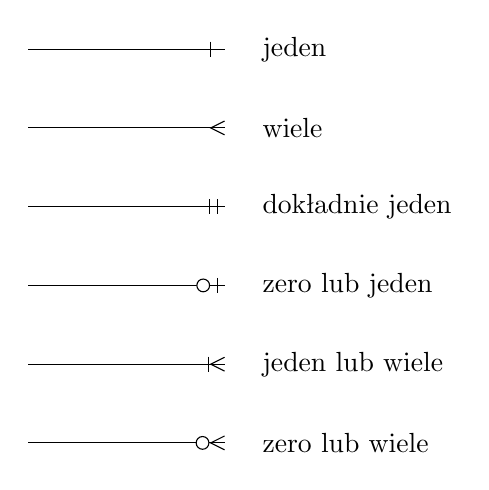
\begin{tikzpicture}
\usetikzlibrary{arrows.meta}

\pgfdeclarearrow{name = No Tip, drawing code=}
\tikzset{
  ER tip sizes/.style n args={3}{
    ER Bar/.tip     ={Bar[width={#2 +1}]},
    ER Circle/.tip  ={Circle[fill={#3}, width={#2}, length={#1}]},
    ER One/.tip     ={ER Bar[sep={#1}] No Tip[]},
    ER Many/.tip    ={Straight Barb[reversed, width={#2}, length={#1}] No Tip[]},
    ER OneOnly/.tip ={ER Bar[sep={(#1)/2}] ER Bar[sep={(#1)/2}] No Tip[]},
    ER ZeroOne/.tip ={ER Circle[sep={(#1)/2}] ER Bar[sep={(#1)/2}] No Tip[]},
    ER OneMany/.tip ={ER Bar[] ER Many[]},
    ER ZeroMany/.tip={ER Circle[] ER Many[]}
  },
  ER tip sizes={+5pt}{+5pt}{white}
}

\draw[arrows=-ER One]      (0,-1) -- ++(right:2.5) node[right]{\quad jeden};
\draw[arrows=-ER Many]     (0,-2) -- ++(right:2.5) node[right]{\quad wiele};
\draw[arrows=-ER OneOnly]  (0,-3) -- ++(right:2.5) node[right]{\quad dokładnie jeden};
\draw[arrows=-ER ZeroOne]  (0,-4) -- ++(right:2.5) node[right]{\quad zero lub jeden};
\draw[arrows=-ER OneMany]  (0,-5) -- ++(right:2.5) node[right]{\quad jeden lub wiele};
\draw[arrows=-ER ZeroMany] (0,-6) -- ++(right:2.5) node[right]{\quad zero lub wiele};
\end{tikzpicture}